\section{Theory} \label{tex:theory}
In this section, the theory used to develop the methods and obtain the result in this thesis will be discussed. First, neural networks (NNs) will be covered - both the simpler artificial NNs (ANNs) and more complex networks such as the convolutional NN (CNN) in both 2 and 3 dimensions. Also methods for calculating the theoretical speed of a NN will be covered. This is followed by the theory behind different methods in tensor decomposition, and how to choose the appropriate rank in some cases.
\begin{figure}[H]
    \centering
    \captionsetup{width=.95\linewidth}
    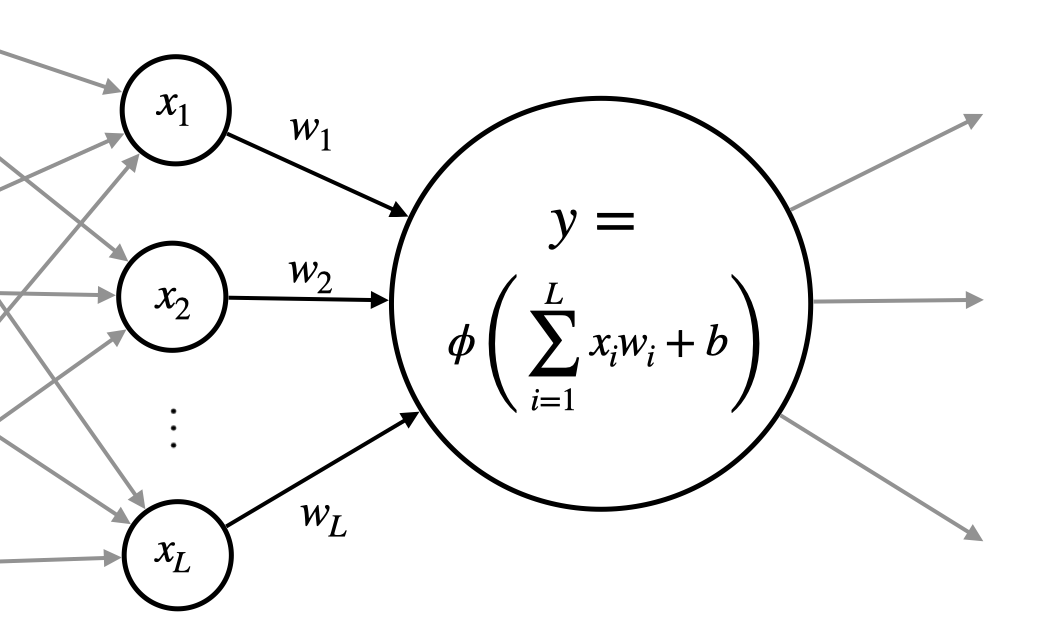
\includegraphics[width=.7\linewidth]{Pics/02_Theory/activation_illustration.png}
    \caption{Illustration of the flow of information through a neuron. Each edge (arrow) has a weight $w$ associated with it, and each neuron (circle) has an activation associated with it. The activations correspond to the information that is passed through the network. $\phi$ is a non-linear transform called the activation function.}
    \label{fig:activation_illustration}
\end{figure}
\subsection{Neural Networks}\label{tex:theory_NN}
The NN is a very useful tool in non-linear classification and regression. It gets its name from what gave rise to the idea of it around half a century ago - the brain. Similar to the brain, a NN consists of a network of neurons that pass on information between each other. The way this is done is illustrated in \autoref{fig:activation_illustration}. Each neuron is, with a given input, associated with a value called its activation. This activation is based on the inputs to that very neuron, and is what is passed on from that neuron. The activation is calculated as the weighted sum of the activations of the inputs to that neuron plus a bias, all non-linearly transformed using an activation function $\phi$. Typical choices of $\phi$ are given in \autoref{fig:activation_functions}, while the typical activation of the last layer (the output) is the softmax-function, given by:
\begin{equation}
\text{Softmax:} \ \ \sigma: \R^K \rightarrow \R^K \qquad \sigma(\bs{x})_i = \frac{e^{x_i}}{\sum_{k=1}^K e^{x_k}} \quad \text{where} \ \bs{x} \in \R^K
\end{equation}
This is due to its ability to ensure a sum of 1 of all the outputs. In the end this value is the probability of the input belonging to each of the output classes. The predicted class is the one that has the highest probability.
\begin{figure}
    \centering
    \captionsetup{width=.95\linewidth}
    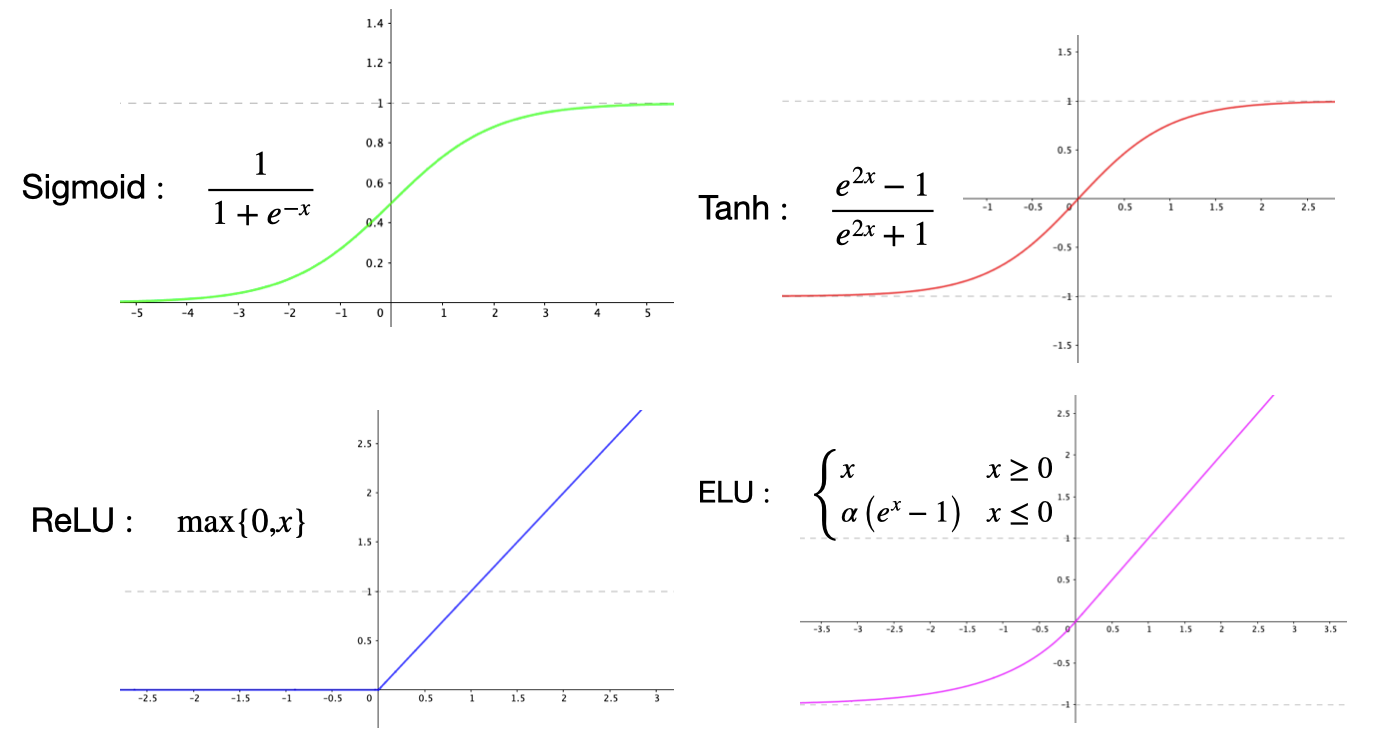
\includegraphics[width=.7\linewidth]{Pics/02_Theory/activation_functions.png}
    \caption{Typical activation functions used in NNs which are all non-linear transforms. The dotted grey lines represent the values of -1 and 1.}
    \label{fig:activation_functions}
\end{figure}

The size and layout of a NN is called the network architecture. The simplest type of NN architecture is the ANN. An example of a very simple ANN with only 2 input values for each observation, and binary output is given in \autoref{fig:very_simple_ANN}. This network has only a single hidden layer with $H$ neurons. 
\begin{figure}
    \centering
    \captionsetup{width=.95\linewidth}
    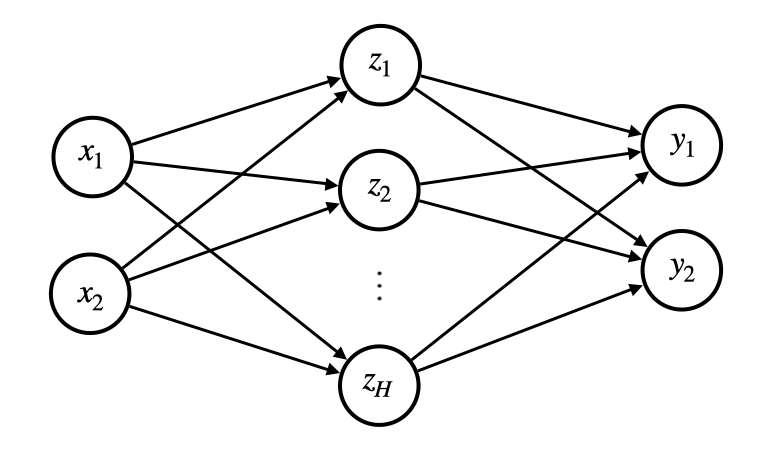
\includegraphics[width=.6\linewidth]{Pics/02_Theory/simple_ANN.png}
    \caption{Illustration of a very simple ANN with only 2 inputs $(x_1, x_2)$, 2 output $(y_1, y_2)$, and a single hidden layer with $H$ neurons $(z_1, z_2,\dots ,z_H)$.}
    \label{fig:very_simple_ANN}
\end{figure}

\subsubsection{Learning}
Learning a NN corresponds to finding the weights of the network that give the highest output accuracy - the best predictions. The method used to find the optimal weights is called back-propagation. This method simply sends inputs through the network and read the outputs. The output error is then propagated backwards through the network in order to adjust the weights accordingly. This is done repeatedly until convergence, normally dividing the training data into smaller batches and performing corrections using every batch. If the amount of data is limited, cross-validation is often used, which trains and validates on the same data. In cross-validation the data is split into a set of folds, and the network is trained on all the data except for one fold which is then used for validating the results.

To represent the error, a so-called loss function is used. Given an observation with input $\bs{x}$ and the corresponding true prediction $y$, we introduce the cost function given by:
\begin{equation}
    L(\Theta | \bs{x},y) = - \hat{p}(y) + \log\left(\sum_{k=0}^K e^{\hat{p}(k)}\right)
\end{equation}
Where $\Theta$ represents all the weights of the network, $K$ is the number of output classes, and $\hat{p}(k)$ is the predicted probability of the input belonging to class $k$. This function is also called the \textit{cross-entropy} loss function and is a the typical choice in classification problems. The cross-entropy loss function can be seen as a function of the weights of the network (here $\Theta$) because the weights are used to find the predictions $\hat{p}$. The gradient of this loss-function with respect to each of the weights in the network is used to update the weights accordingly by a gradient-descent step:
\begin{equation}
    \Theta_{new} = \Theta - \gamma \ \nabla L (\Theta)
\end{equation}
Where $\gamma$ is the learning rate that can be used to determine the speed of the learning, i.e. bigger values implies bigger jumps, while smaller values are used for fine-tuning. This derivative can be found either analytically, by applying the chain rule backwards through the network, or automatically using the \textit{autograd}-function in \textit{PyTorch}. In this thesis the \textit{autograd}-function will be used to find the derivatives, hence for the analytical derivations cf. \cite{elements_NN} or \cite{Zhang2016}.

\subsubsection{Architectures}
NNs are very flexible and can easily be adapted to fit every need. Not only can they be built off an arbitrary number of layers of different sizes, but also there are multiple different types of layers. Each layer finds progressively more complex features in the input data, hence more layers will be able to find more complex features. NNs can be both feed-forward (information flows forward) or recurrent (information flows backwards). The two types of layers that we will cover in this thesis are the dense layer and the convolutional layer respectively. Both have powerful properties and will be discussed further in the following.

\paragraph{The dense layer}
The dense layer is the basic building block of NNs, and ANNs are almost always built of these. A dense layer (also called fully-connected layer) is a layer in which each of neurons have a connection with all the neurons in the previous layer. Both the middle and output layers in the network illustrated in \autoref{fig:very_simple_ANN} are dense layers. In CNNs the dense layers are often used in the last part of the network to condense the information from the convolutional layers.

The dense layer is calculated as the non-linear transform of a matrix-vector product with the matrix consisting of the weights on the edges connecting the layer to the previous, and the vector being the input from the previous layer. This concept is illustrated in \autoref{fig:dense_layer_VM_prod}.
\begin{figure}
    \centering
    \captionsetup{width=.95\linewidth}
    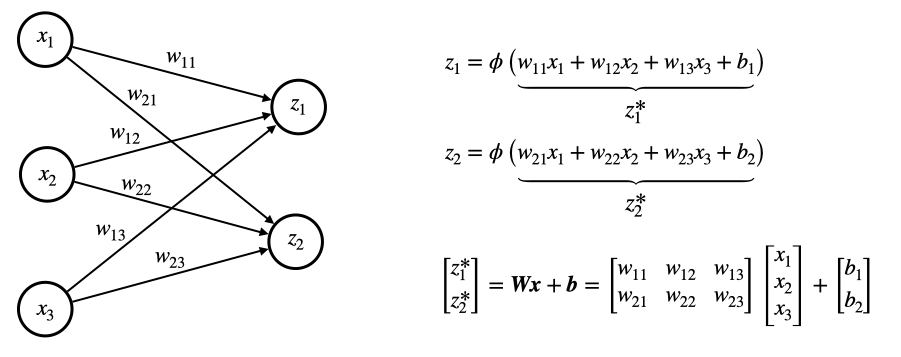
\includegraphics[width=\linewidth]{Pics/02_Theory/dense_layer_VM_prod.png}
    \caption{Illustration of the calculation of the dense layer. The dense layer is calculated as the non-linear transform of the bias plus the matrix-vector product between the weights and the input vector. $\phi$ is the activation function or non-linear transform.}
    \label{fig:dense_layer_VM_prod}
\end{figure}

\paragraph{The convolutional layer}
The convolutional layer has become a very powerful tool in image classification due to its ability to find features in images using the spatial information. 

\subsection{Decomposition Methods}\label{tex:decomp_methods}